% !TEX root = Bachelorarbeit Synthetische Daten.tex
\chapter{Ergebnisse} \label{ch:results}

Dieses Kapitel präsentiert die Ergebnisse der Arbeit. Es wird auf die generierten synthetischen Daten eingegangen und die Trainings- und Testergebnisse der Modelle beschrieben. Anschließend wird die Klassifikations-Performance und Out-of-Distribution-Detektion aus den drei Versuchsreihen in Bezug auf die Forschungsfragen miteinander verglichen.

\section{Die generierten synthetischen Daten} \label{sec:da-fusion-results}

% Einleitung
Im Rahmen der Untersuchung wurden sowohl In-Distribution als auch Near Out-of-Distribution-Augmentationen mit DA-Fusion generiert. Dieser Abschnitt bewertet die Qualität dieser Augmentationen und untersucht sowohl positive als auch negative Beispiele. Es wird insbesondere auf die visuelle Überzeugungskraft, die semantische Konsistenz und mögliche Artefakte eingegangen, die während des Generierungsprozesses aufgetreten sind.

\subsection{In-Distribution-Augmentationen} \label{subsec:da-fusion-id-results}

Die synthetischen In-Distribution-Daten, die durch DA-Fusion generiert wurden, zeigten überwiegend eine hohe Qualität. Einige Beispiele sind in Anhang \ref{sec:app2}, \autoref{fig:id-augs-good-1} und \ref{fig:id-augs-good-2} zu sehen.

Die Bilder wirken zum größten Teil überzeugend und realistisch. Die Unterschiede sind auf den ersten Blick sehr subtil, vor allem, wenn die Bilder Seite an Seite betrachtet werden. Dennoch sind Veränderungen in der Textur der Oberflächen erkennbar, etwa unterschiedliche Verteilungen von Rost und Verschmutzung.

Insgesamt ist durch rein visuelle Inspektion also keine auffällige Veränderung in der Beschaffenheit oder des Gebrauchszustands der Objekte zu erkennen. Trotzdem werden diese Zustände in einer breiteren Palette von Variationen dargestellt.

In einigen Fällen sind die Ergebnisse jedoch weniger überzeugend. In Anhang \ref{sec:app2}, \autoref{fig:id-augs-bad} sind Beispiele für mangelhafte In-Distribution-Daten zu sehen. Die synthetischen Objekte sind in diesen Fällen nicht realistisch und weisen deutliche Artefakte auf. Oftmals hängt die Qualität der Daten mit Größe des Objektes im Originalbild zusammen (was auch die Auflösung des ROI-Crops entscheidet). Bei kleineren Objekten fällt die Augmentation relativ gesehen stärker aus, was zu einer stärkeren Verzerrung führen kann.

Insgesamt lässt sich feststellen, dass die Mehrheit der ID-Augmentationen als realistisch wahrgenommen werden und die Variation erhöhen.

\subsection{Near Out-of-Distribution-Augmentationen} \label{subsec:da-fusion-ood-results}

Die Near Out-of-Distribution-Augmentationen zeigten im Vergleich zu den ID-Daten eine gemischtere Qualität. Beispiele sind in Anhang \ref{sec:app2}, \autoref{fig:ood-augs-good} zu sehen.

Die meisten Objekte wirken etwas weniger realistisch, aber dennoch plausibel. Vor allem ist hier der Einfluss der unterschiedlichen Text-Prompts zur Augmentation deutlicher erkennbar, wodurch die Objekte in mit mehr Variation in den Gebrauchtzuständen dargestellt werden.

Allerdings gibt es hier deutlich mehr Beispiele, die weniger überzeugend sind (siehe Anhang \ref{sec:app2}, \autoref{fig:ood-augs-bad}). Die synthetischen Objekte weisen in diesen Fällen deutliche Artefakte auf oder sind vollständig vom ursprünglichen Konzept entkoppelt.

Zusammenfassend ist die Qualität der OOD-Augmentationen also weniger konsistent als die der ID-Augmentationen. Die Variationen sind zwar größer, aber auch die Qualitätsschwankungen sind stärker.

\section{Trainings- und Testergebnisse} \label{sec:supcon-results}

% Einleitung
Nachfolgend werden die Ergebnisse der Trainings- und Testdurchläufe im Supervised Contrastive Learning beschrieben. Die Betrachtung umfasst die Trainingskurven, den Verlauf des Validierungsfehlers sowie die finale Leistung der Modelle auf den Validierungsdaten. Besondere Aufmerksamkeit liegt auf der Evaluation der Klassifikationsgenauigkeit (Accuracy) und der Fähigkeit, OOD-Daten zu erkennen.

\subsection{Contrastive Pre-Training} \label{subsec:supcon-pre-results}

Die Trainingskurven des Contrastive Pre-Trainings sind in \autoref{fig:supcon-pre-loss} dargestellt. Die Trainings- und Validierungsfehler zeigen insgesamt eine gute Konvergenz, wobei zu erkennen ist, dass der Validierungsfehler im Vergleich zum Trainingsfehler etwas höher und weniger stabil ist, was auf ein gewisses Overfitting des Modells auf die Trainingsdaten hindeuten könnte.

\begin{figure}[h]
	\centering
	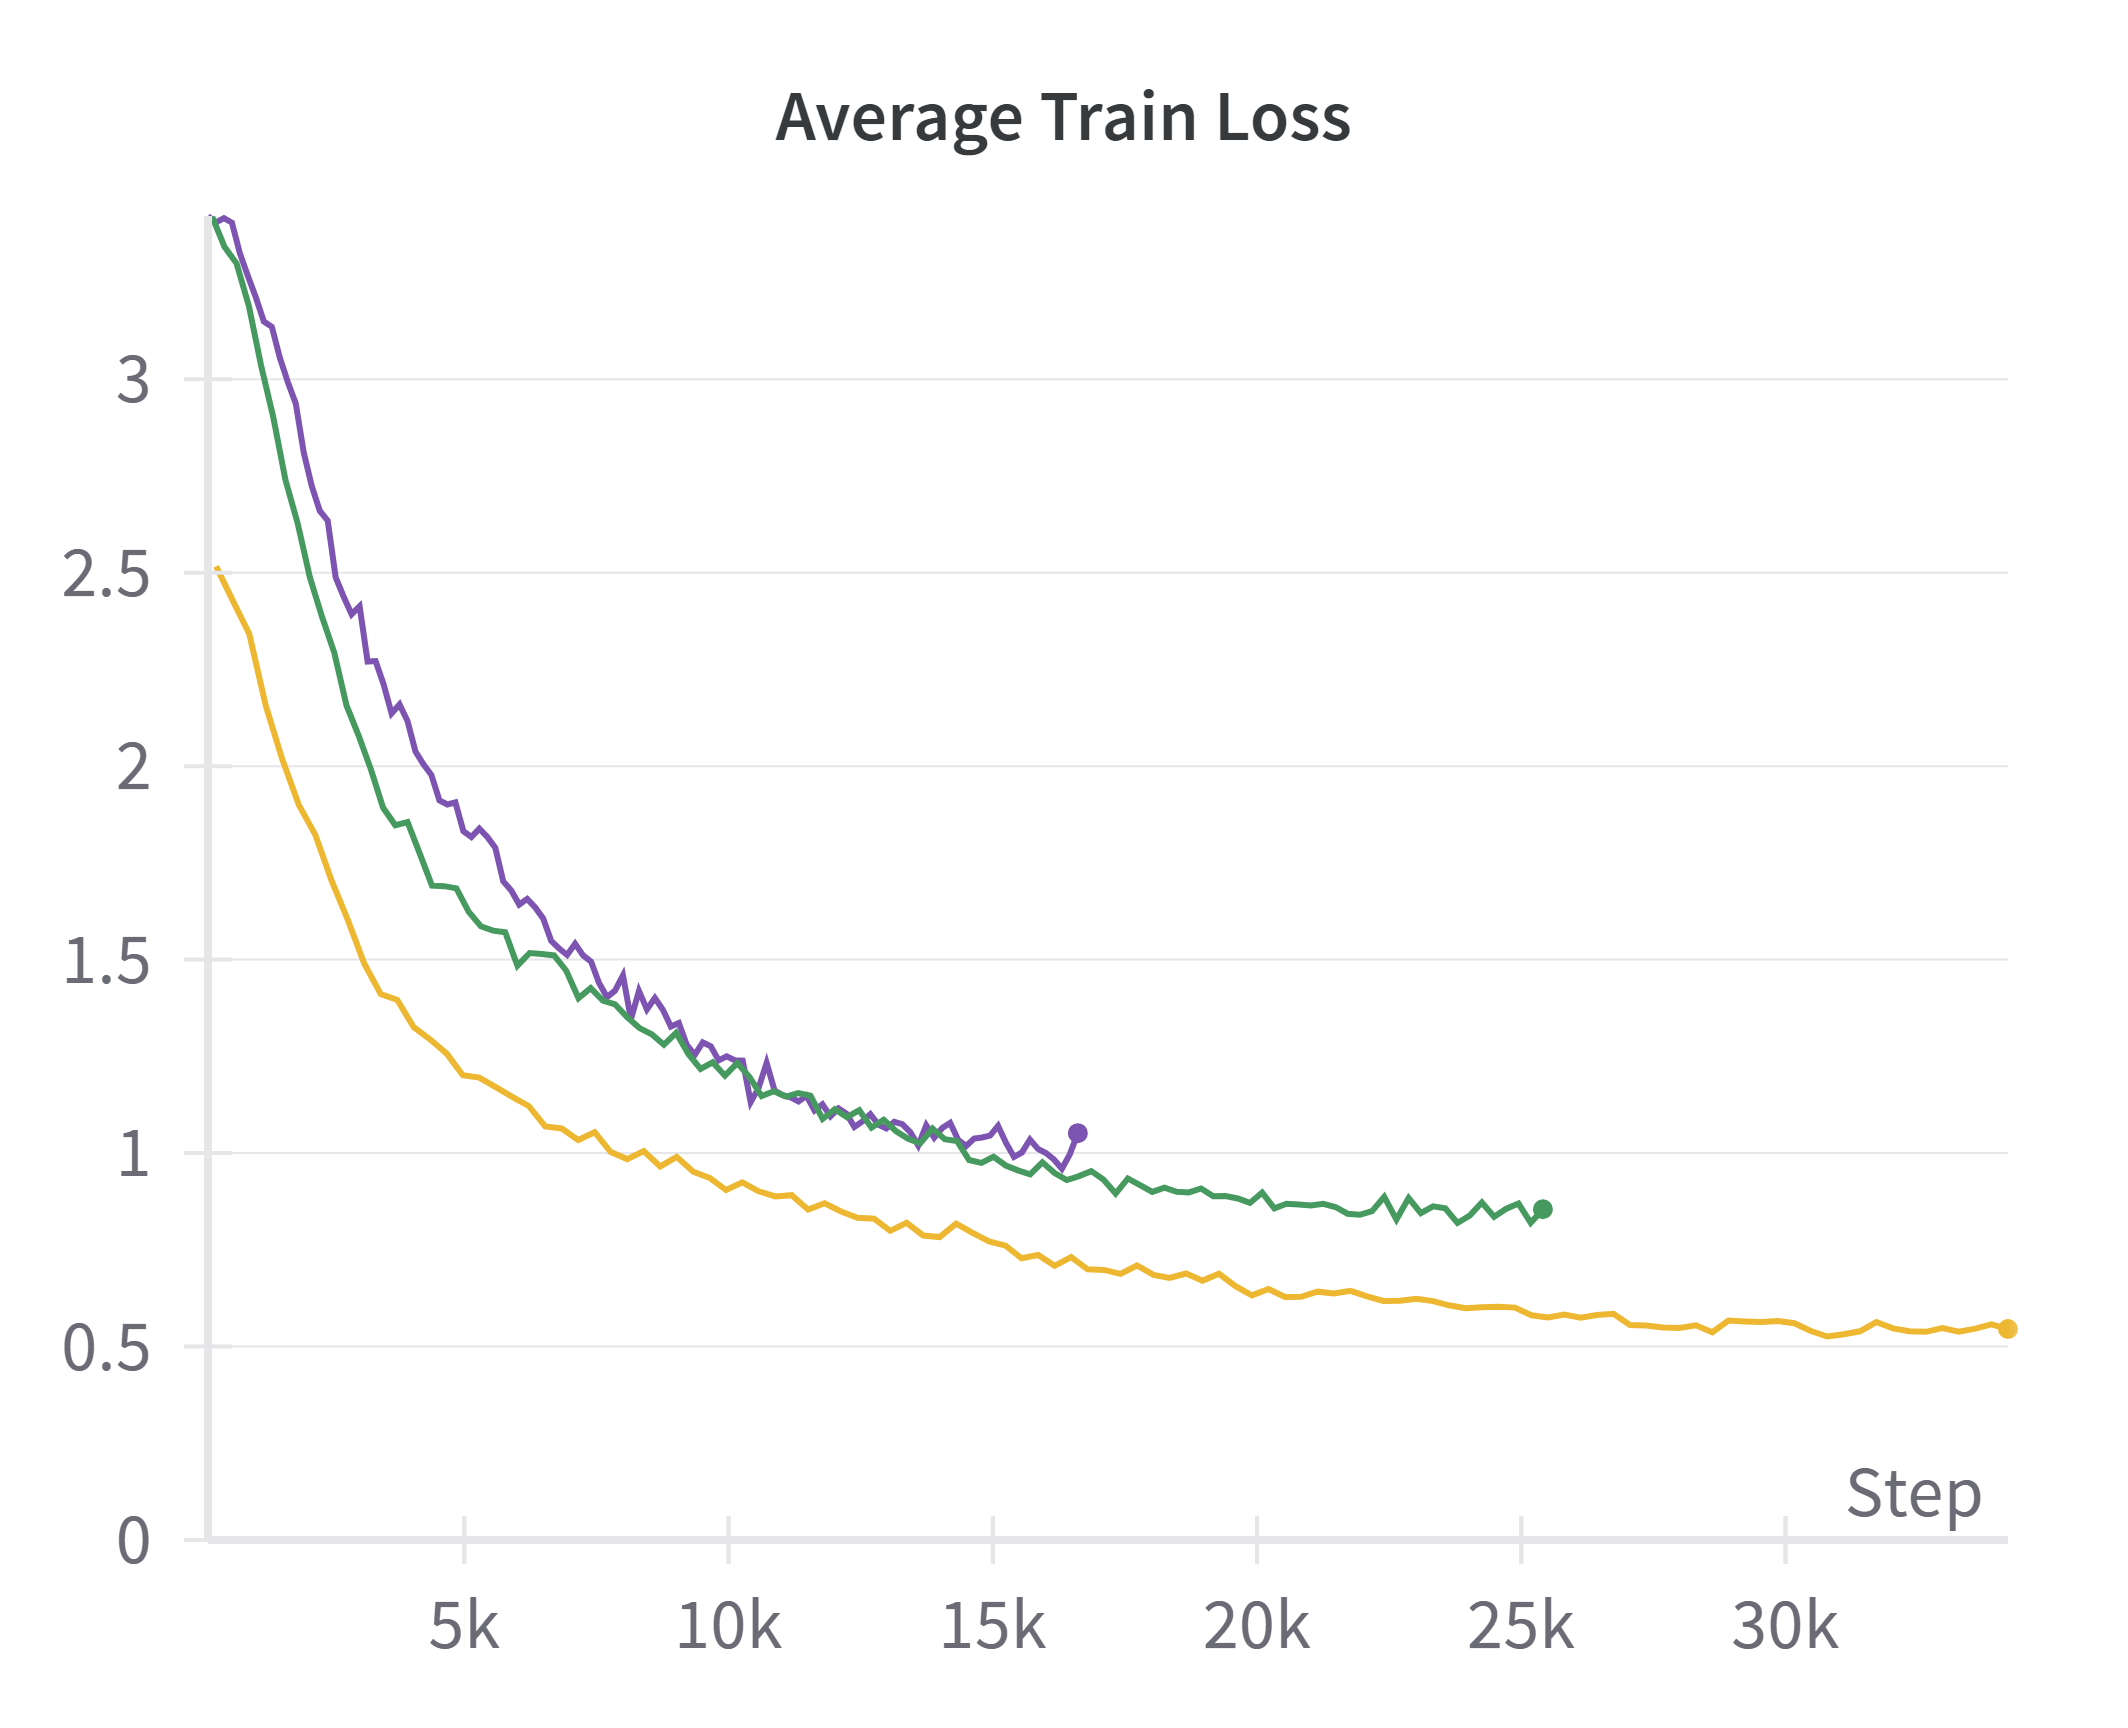
\includegraphics[width=0.5\textwidth]{images/figure_results_supcon-pre_avg-train-loss.png}%
	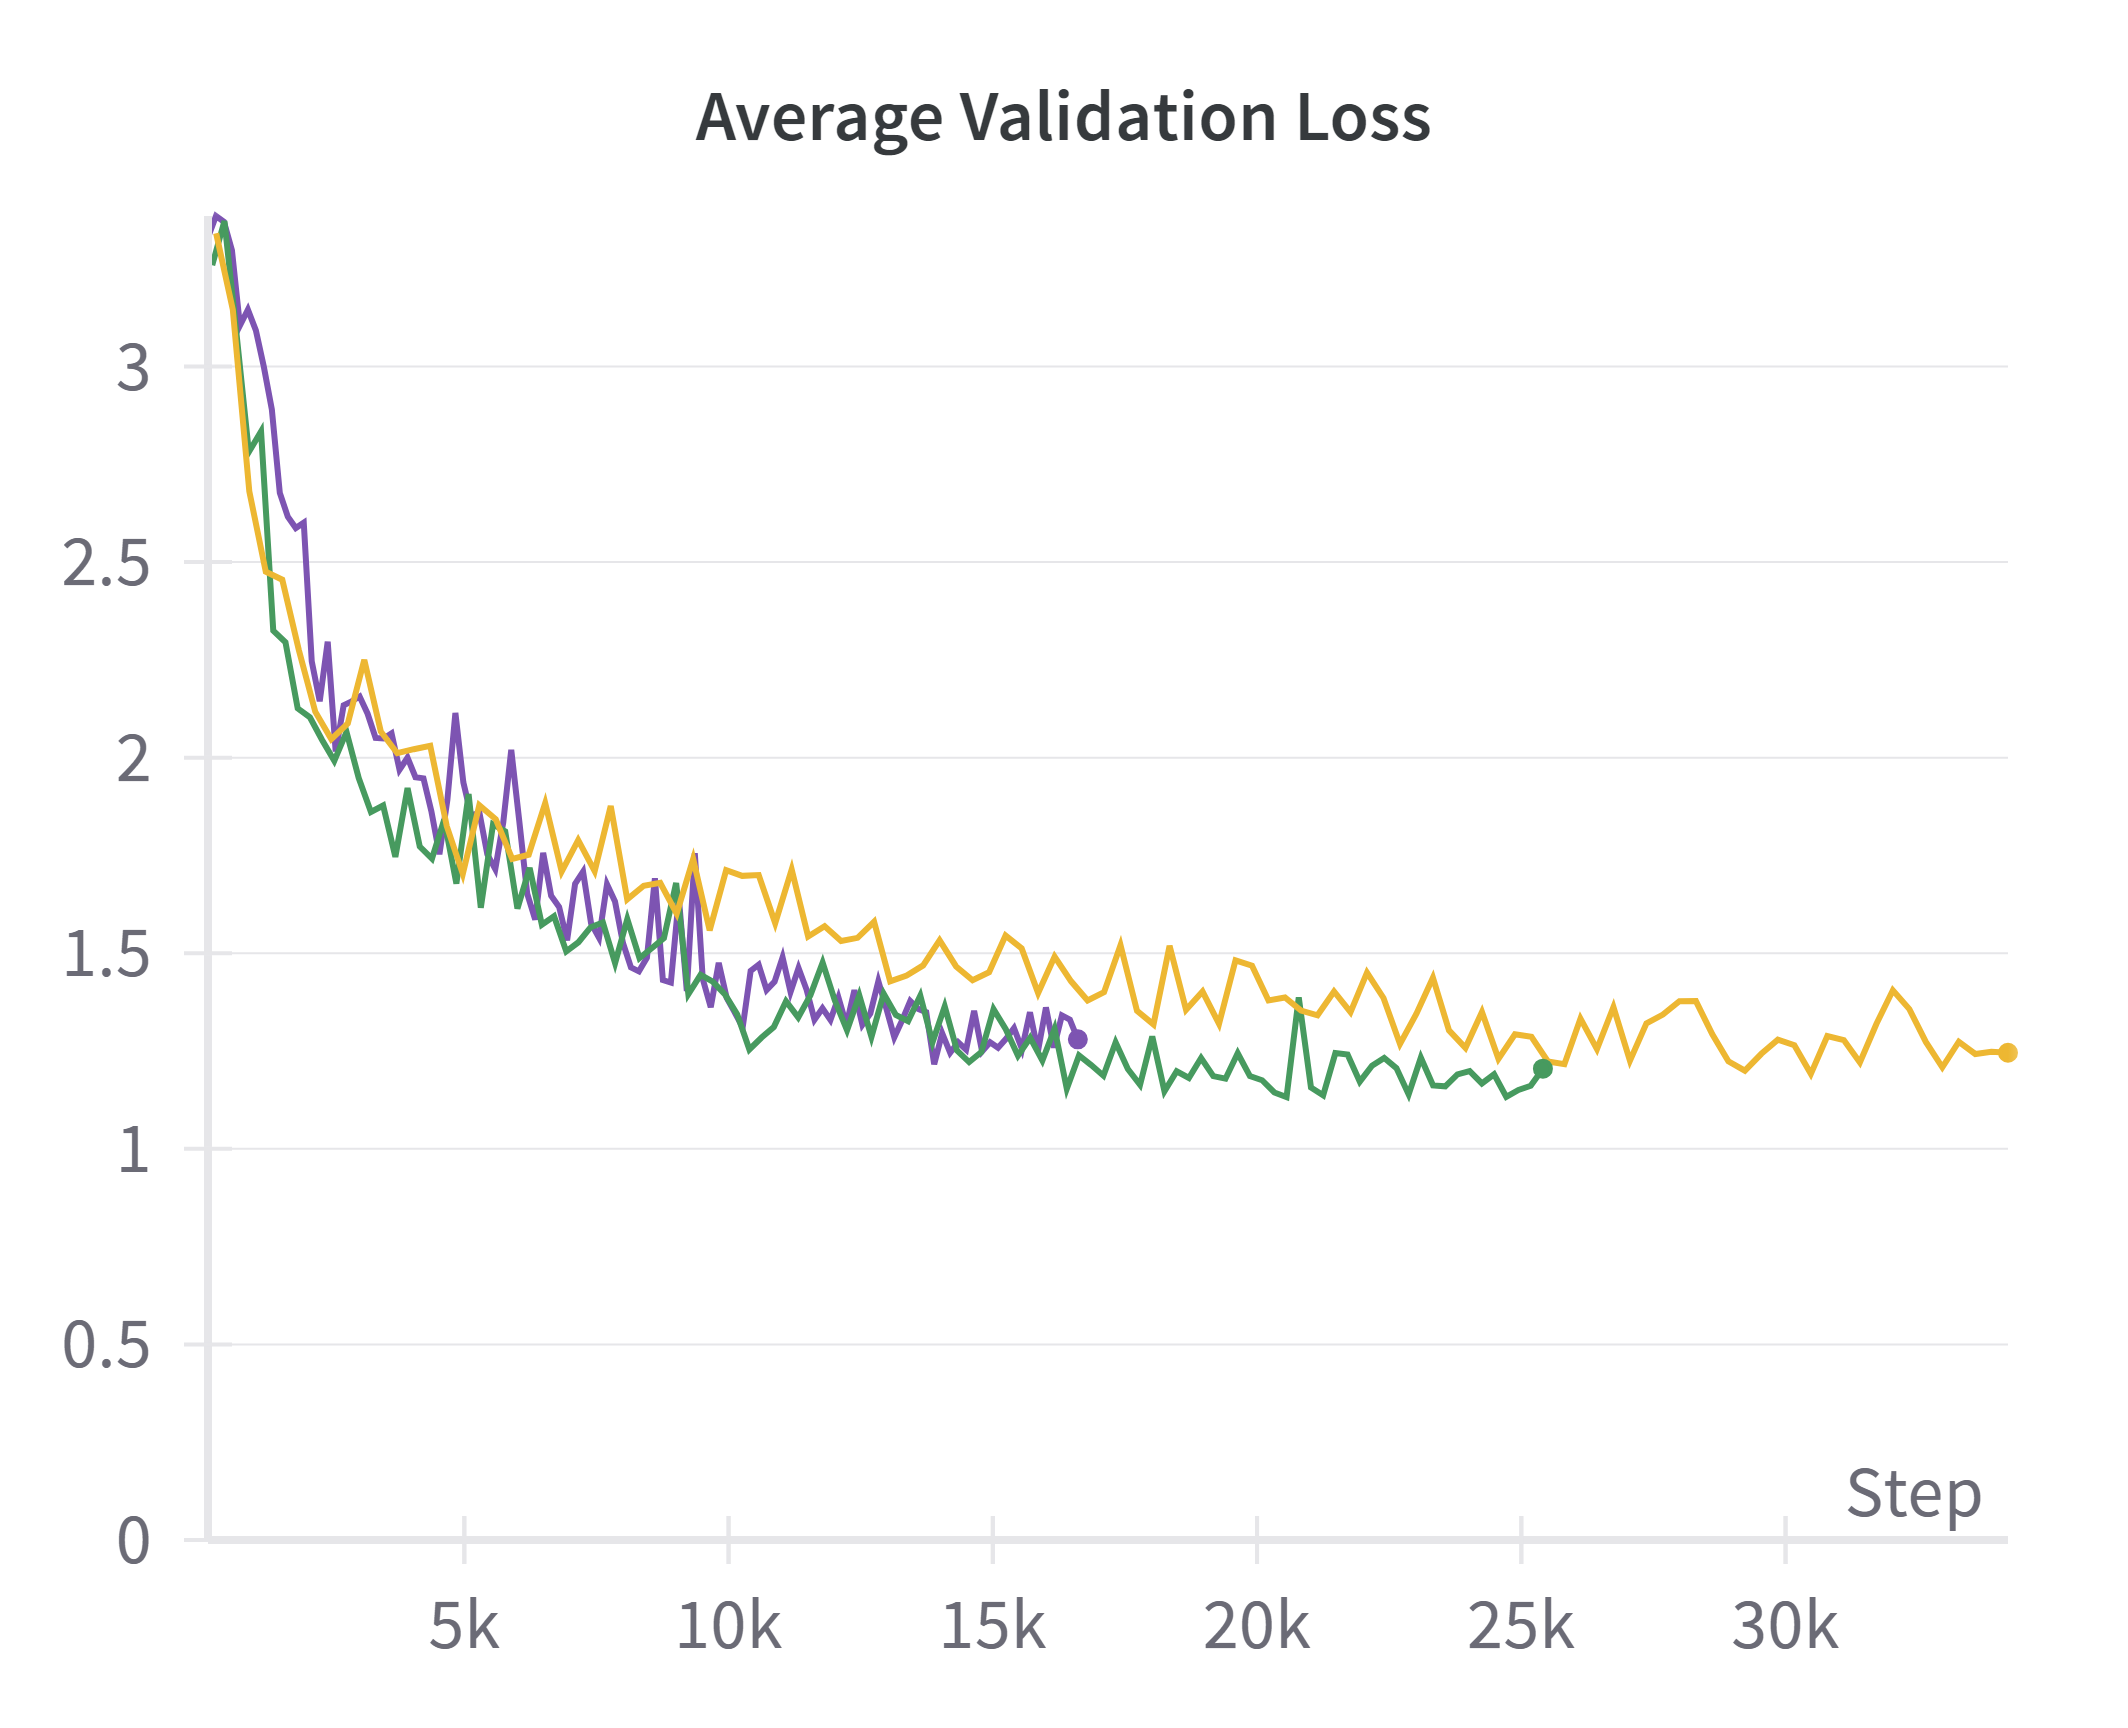
\includegraphics[width=0.5\textwidth]{images/figure_results_supcon-pre_avg-val-loss.png}
	\caption[Trainings- und Validierungsfehler während des Contrastive Pre-Trainings.]{Trainings- und Validierungsfehler während des Contrastive Pre-Trainings (\textcolor{exp1}{Lila}: Versuch 1, \textcolor{exp2}{Grün}: Versuch 2, \textcolor{exp3}{Gelb}: Versuch 3).}
	\label{fig:supcon-pre-loss}
\end{figure}

% Leichte Verbesserung bei Versuch 2
Beim Vergleich der Versuche fällt auf, dass die Trainings- und Validierungsfehler in Versuch 2 nahezu identisch mit denen in Versuch 1 verlaufen. Durch die zusätzlichen Augmentationen läuft das Training in Versuch 2 jedoch ein wenig länger, sodass die Performance sich weiter verbessert.

% Leichte Verschlechterung bei Versuch 3
Versuch 3 zeigt auf den Trainingsdaten einen insgesamt signifikant niedrigeren Fehler, während der Fehler auf den Validierungsdaten bis zum Ende des Trainings etwas höher ist als bei den anderen Versuchen, trotz der längsten Trainingsdauer.

\subsection{Lineare Klassifikation} \label{subsec:supcon-lin-results}

Die lineare Klassifikation der im vorherigen Schritt erlernten Repräsentationen zeigt ebenfalls interessante Trends. In \autoref{tab:supcon-lin-results} sind die finalen Testergebnisse auf den Validierungsdaten zusammengefasst, während die Trainingskurven in \autoref{fig:supcon-lin-loss} (Fehler), \autoref{fig:supcon-lin-acc} (Top-1 Accuracy) und \autoref{fig:supcon-lin-ood-detection} (ID- und OOD-Confidence) zu sehen sind.

\begin{table}[h]
	%\centering
	\caption{Die finalen Testergebnisse der linearen Klassifikation auf den Validierungsdaten.}
	\begin{tabular}{|c|c|c|}
		\hline
		\textbf{Versuch} & \textbf{Top-1 Accuracy} & \textbf{ID-/OOD-Confidence ($\Delta$)} \\
		\hline
		1 & 71.4\% & 0.69 / 0.62 (0.07) \\
		2 & 77.5\% & 0.76 / 0.65 (0.11) \\
		3 & 75.3\% & 0.40 / 0.35 (0.05) \\
		\hline
	\end{tabular}
	\label{tab:supcon-lin-results}
\end{table}

\newpage

\begin{figure}[h]
	\centering
	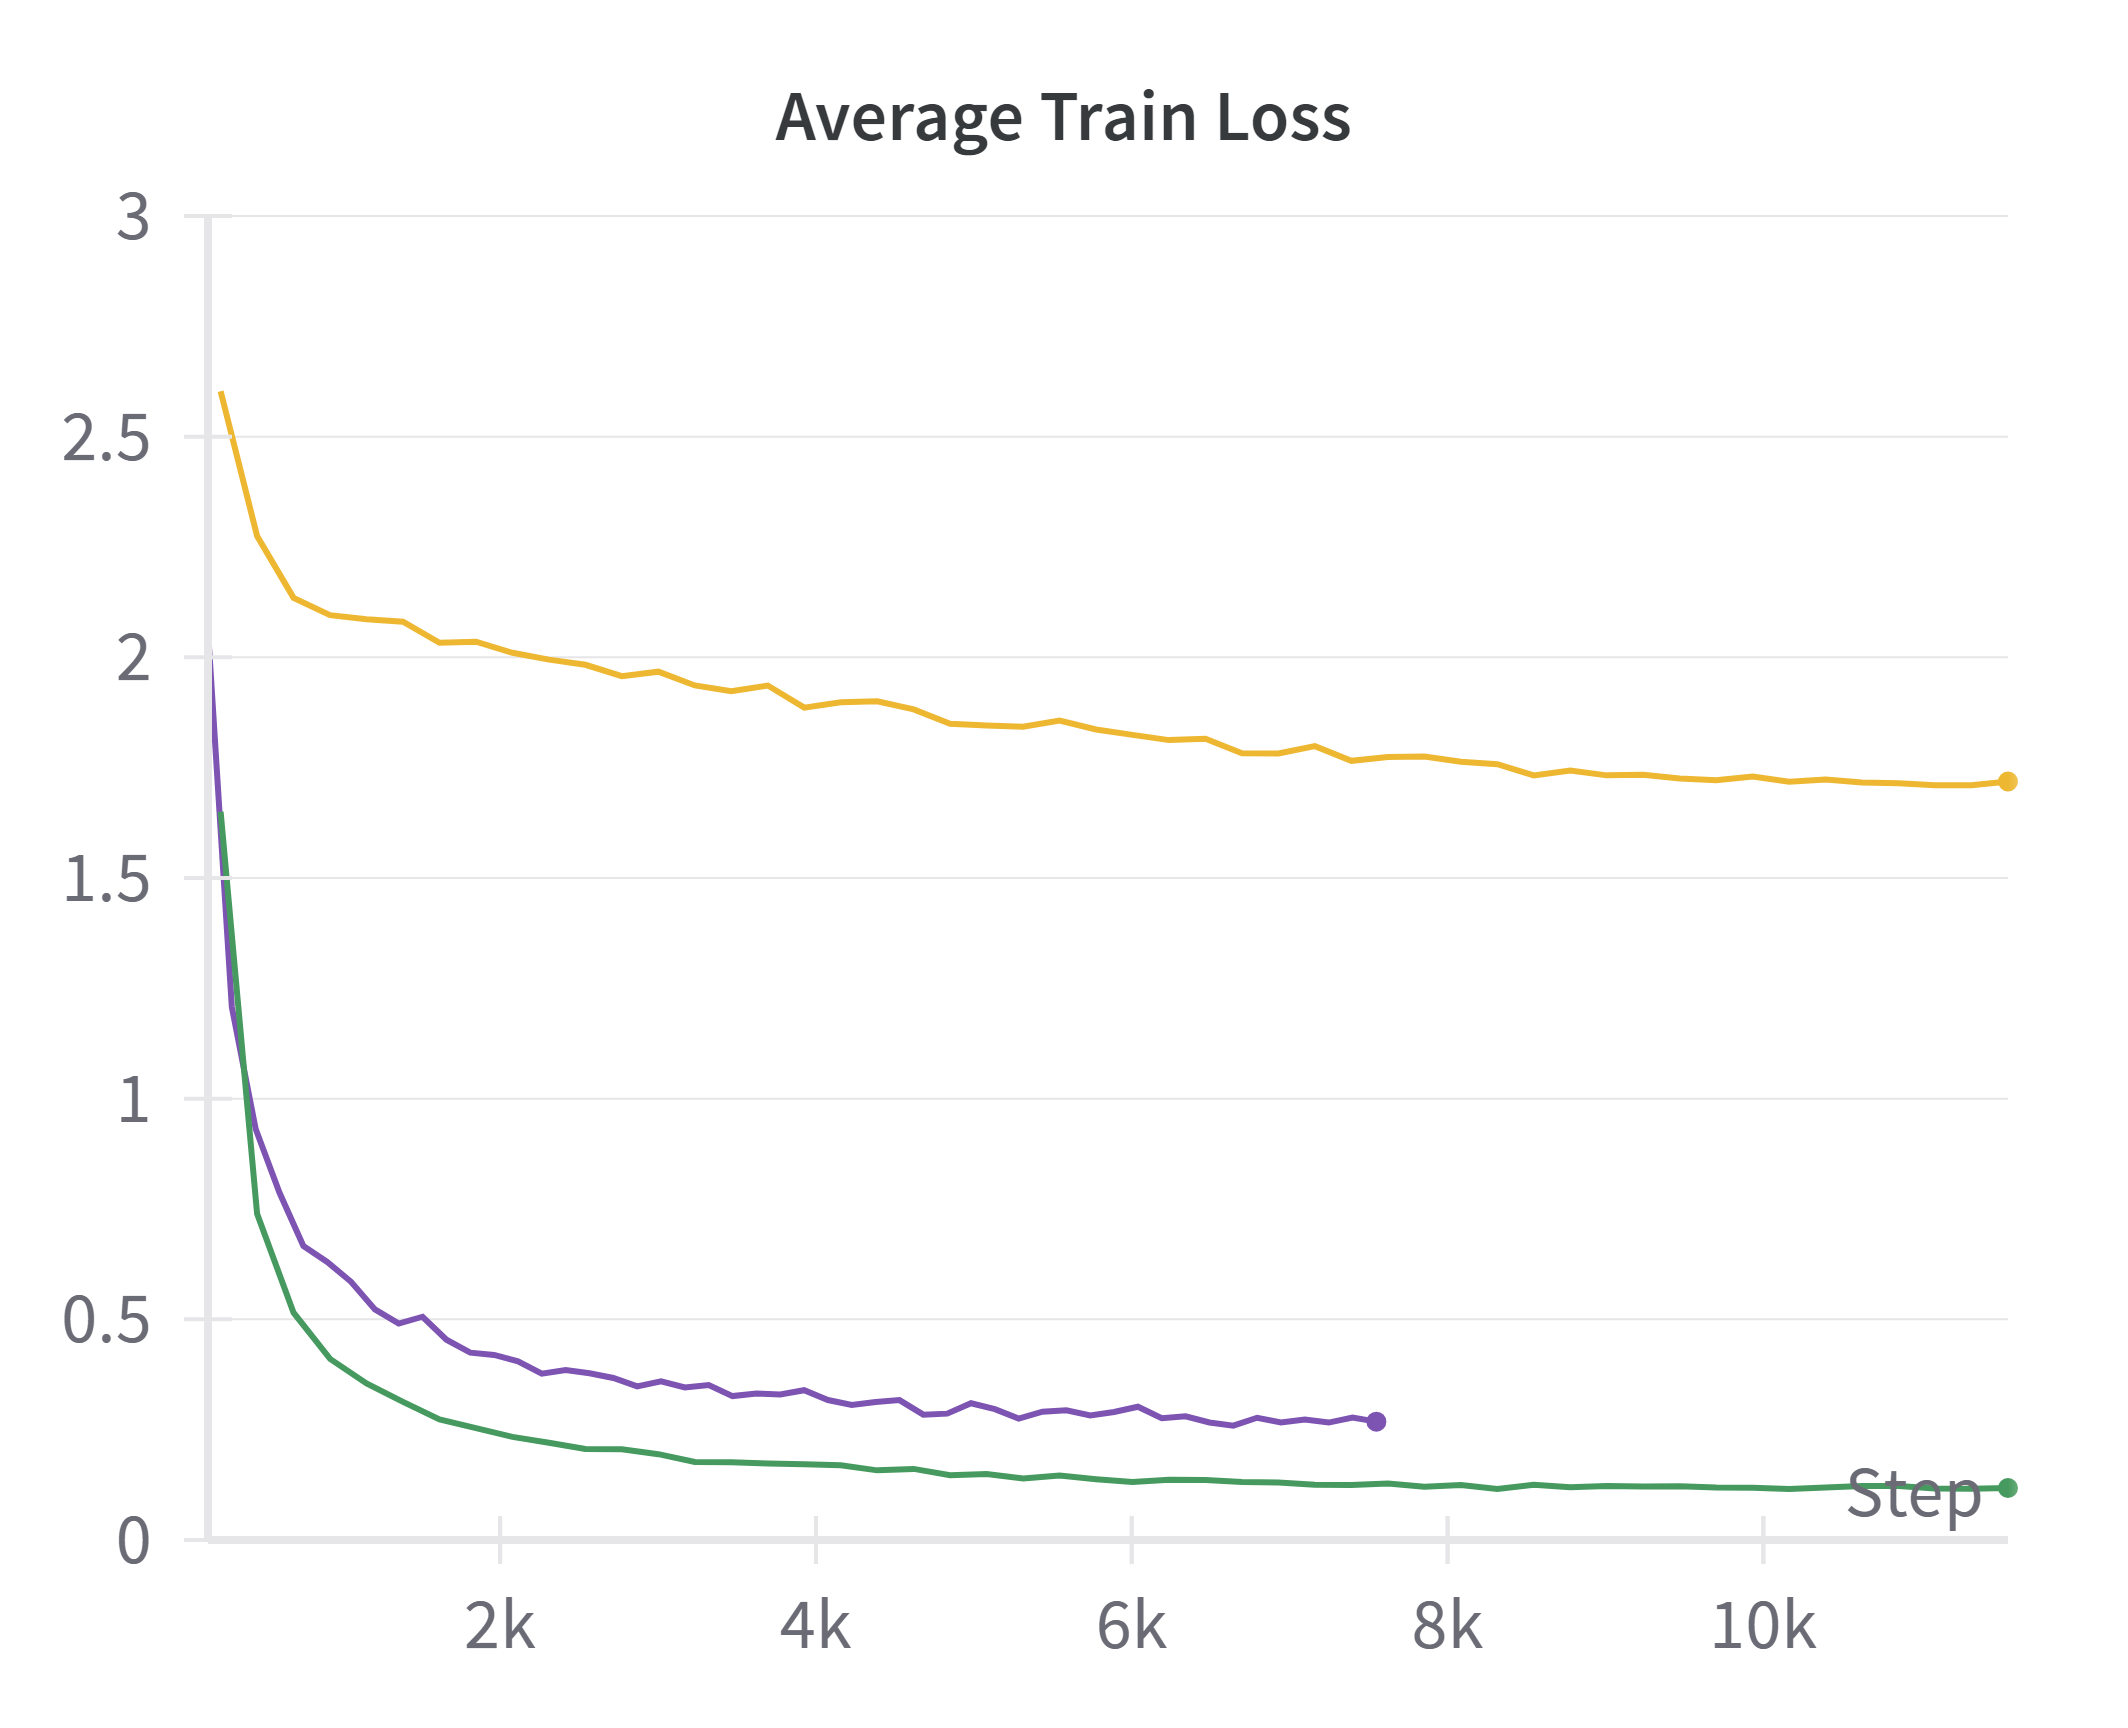
\includegraphics[width=0.5\textwidth]{images/figure_results_supcon-lin_avg-train-loss.png}%
	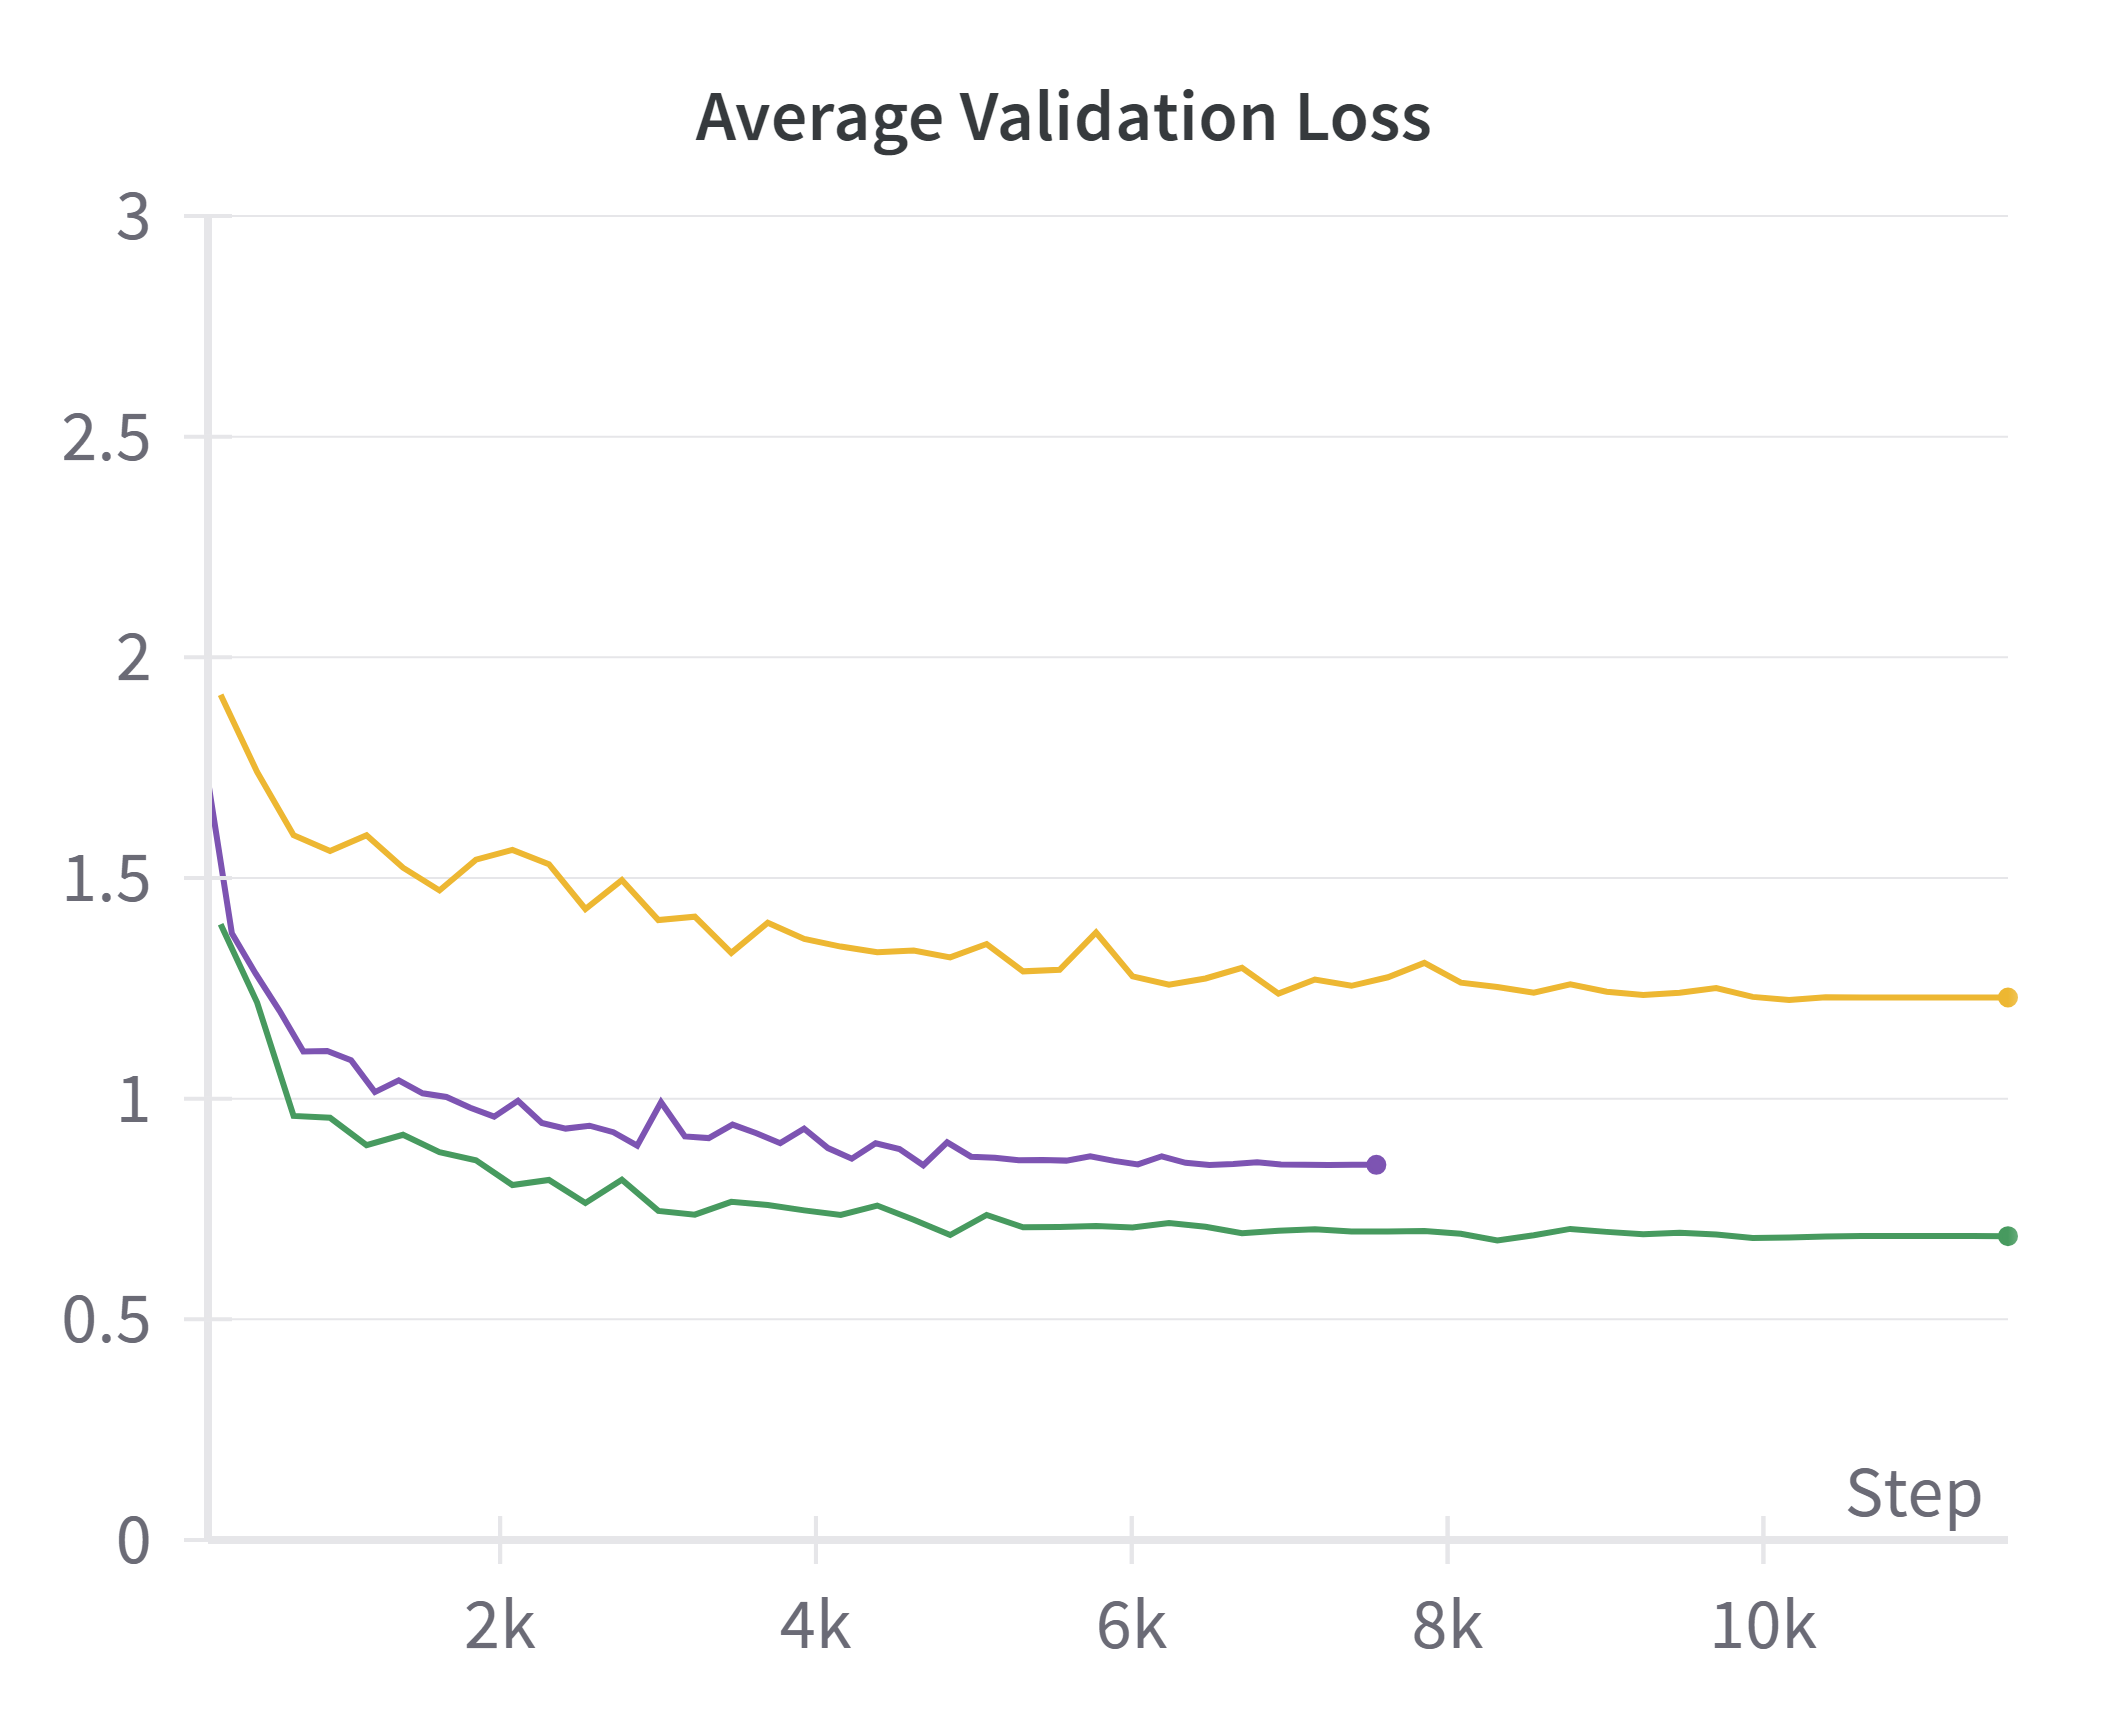
\includegraphics[width=0.5\textwidth]{images/figure_results_supcon-lin_avg-val-loss.png}
	\caption[Trainings- und Validierungsfehler der linearen Klassifikation.]{Trainings- und Validierungsfehler der linearen Klassifikation (\textcolor{exp1}{Lila}: Versuch 1, \textcolor{exp2}{Grün}: Versuch 2, \textcolor{exp3}{Gelb}: Versuch 3).}
	\label{fig:supcon-lin-loss}
\end{figure}

% Viel höherer Fehler bei Versuch 3
Die Trainingskurven zeigen sehr geringe Trainingsfehler für Versuche 1 und 2, aber einen viel höheren Fehler bei Versuch 3. Die Validierungsfehler der Versuche nähern sich wieder etwas an, wobei weiterhin ein deutlicer Abstand zwischen Versuch 3 und den anderen Versuchen besteht. Während der Validierungsfehler bei den Versuchen 1 und 2 also höher ist als der Trainingsfehler, ist es bei Versuch 3 umgekehrt.

\begin{figure}[h]
	\centering
	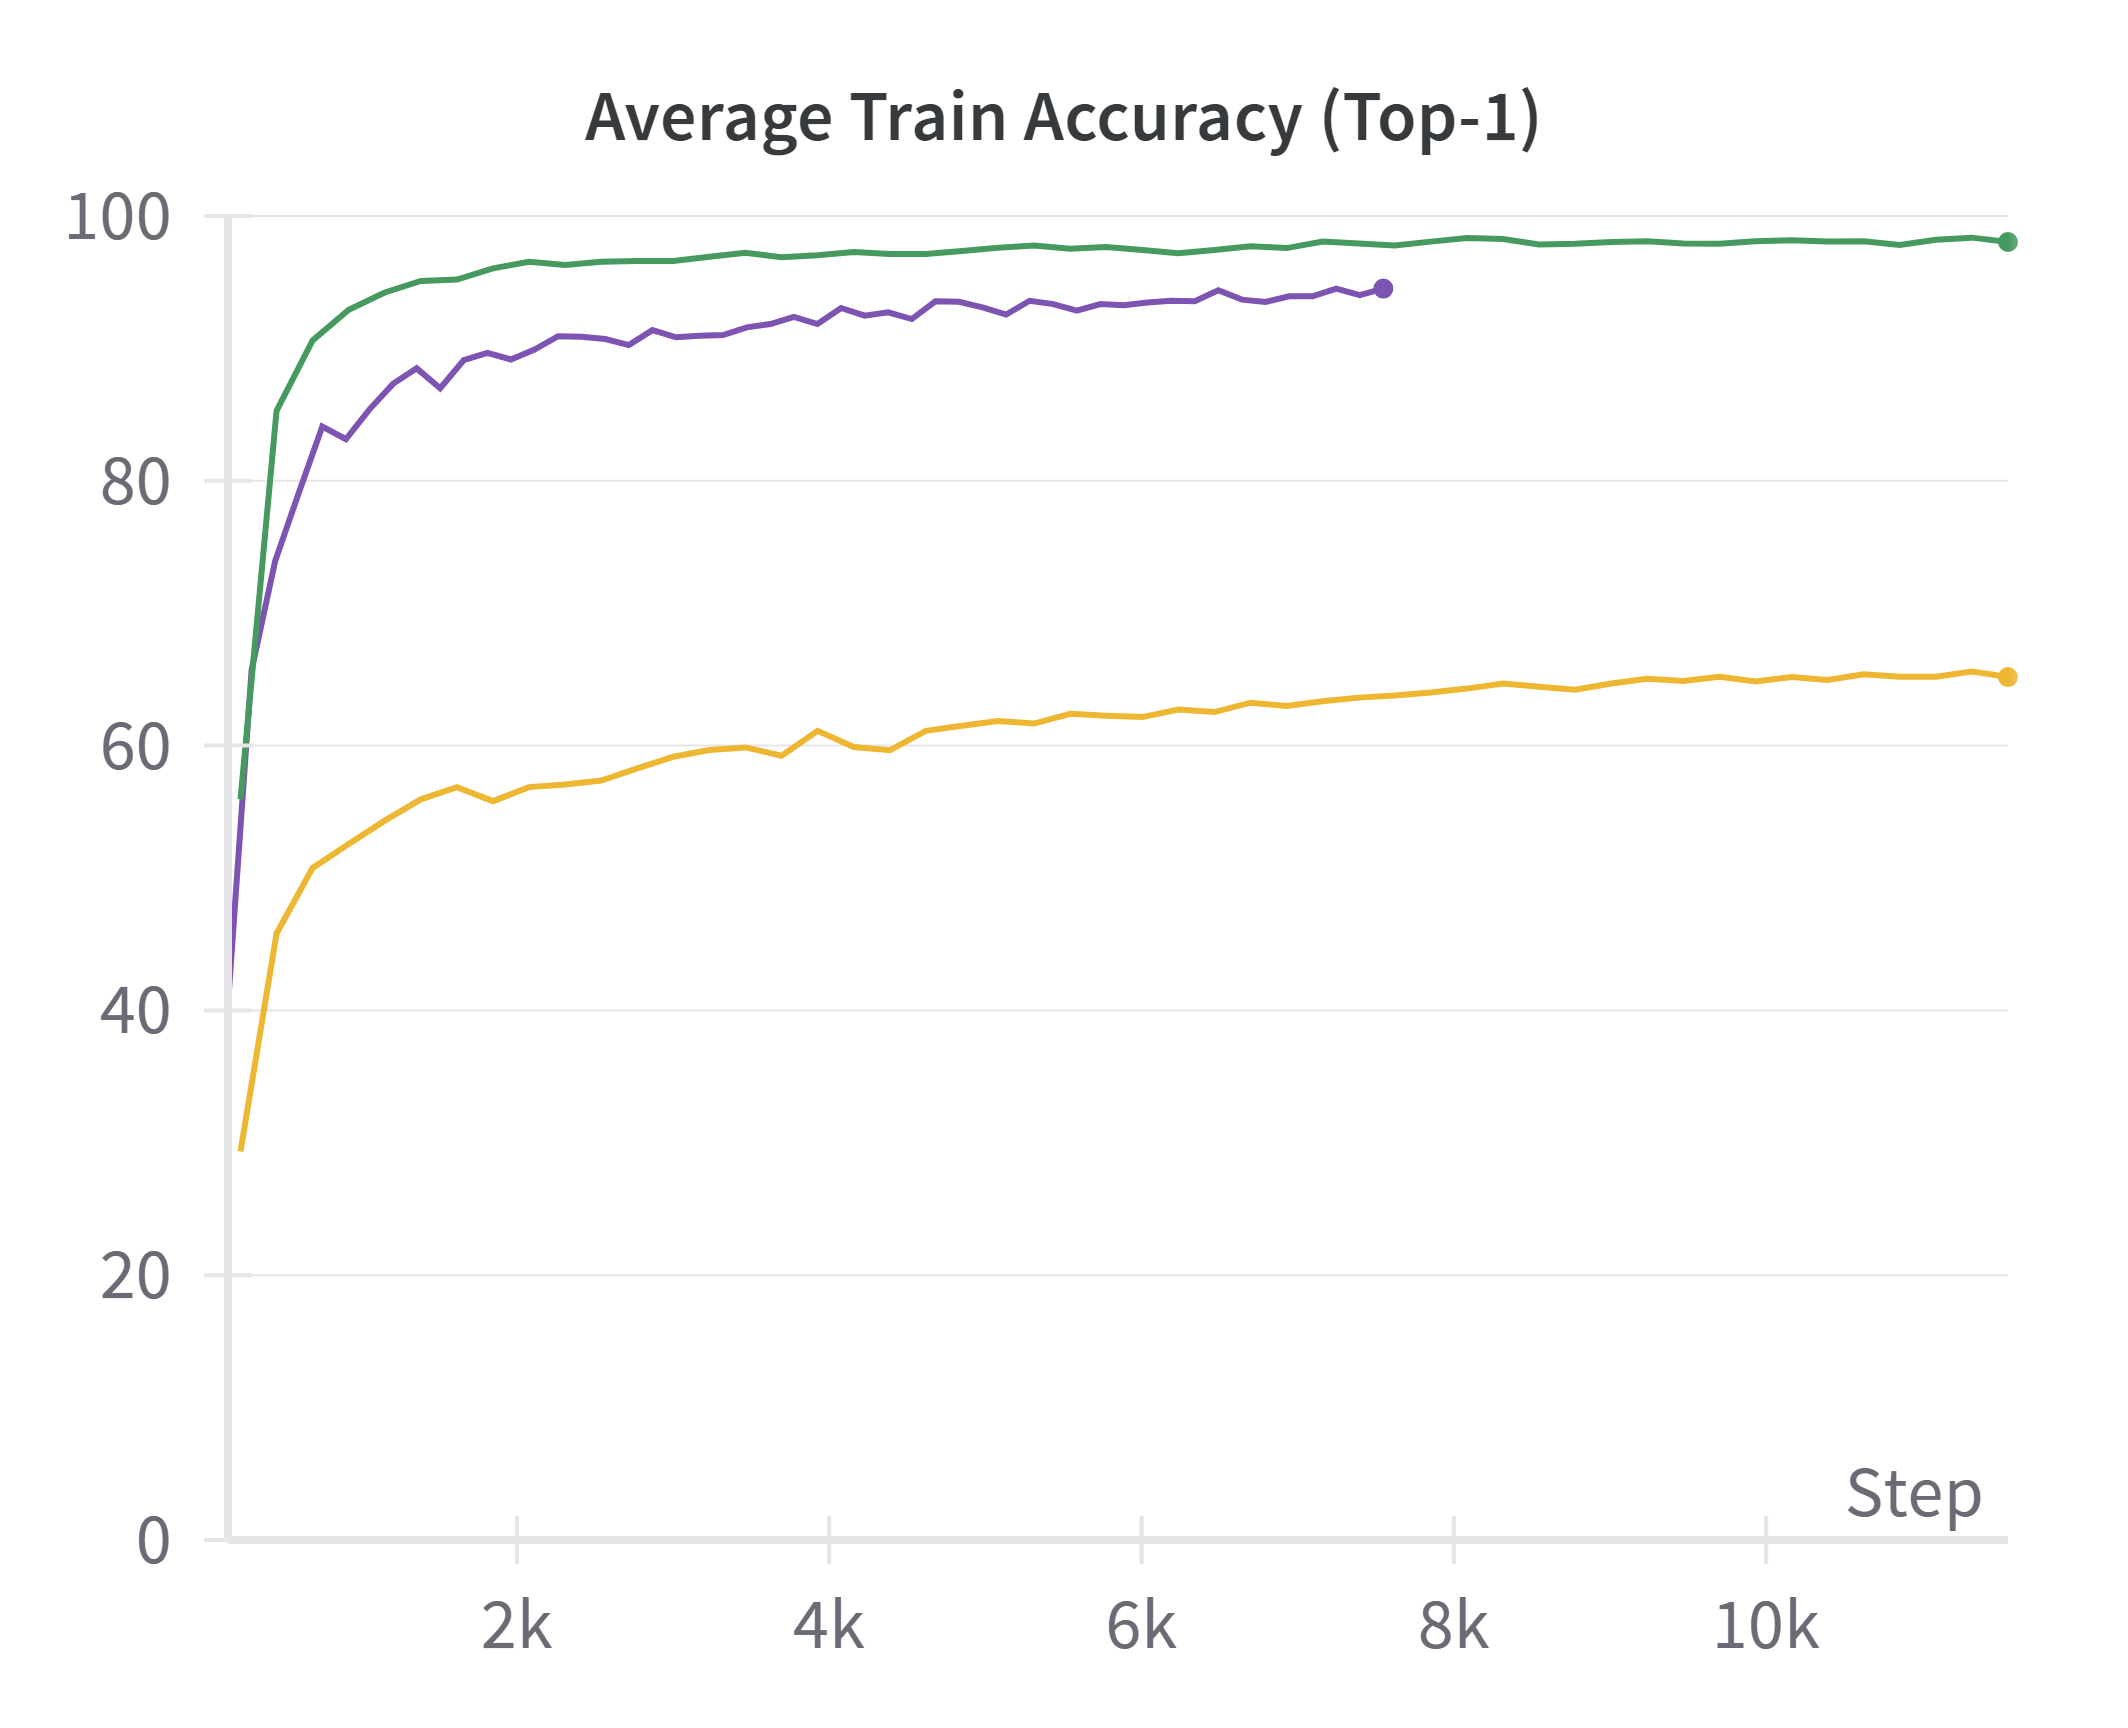
\includegraphics[width=0.5\textwidth]{images/figure_results_supcon-lin_avg-train-acc.png}%
	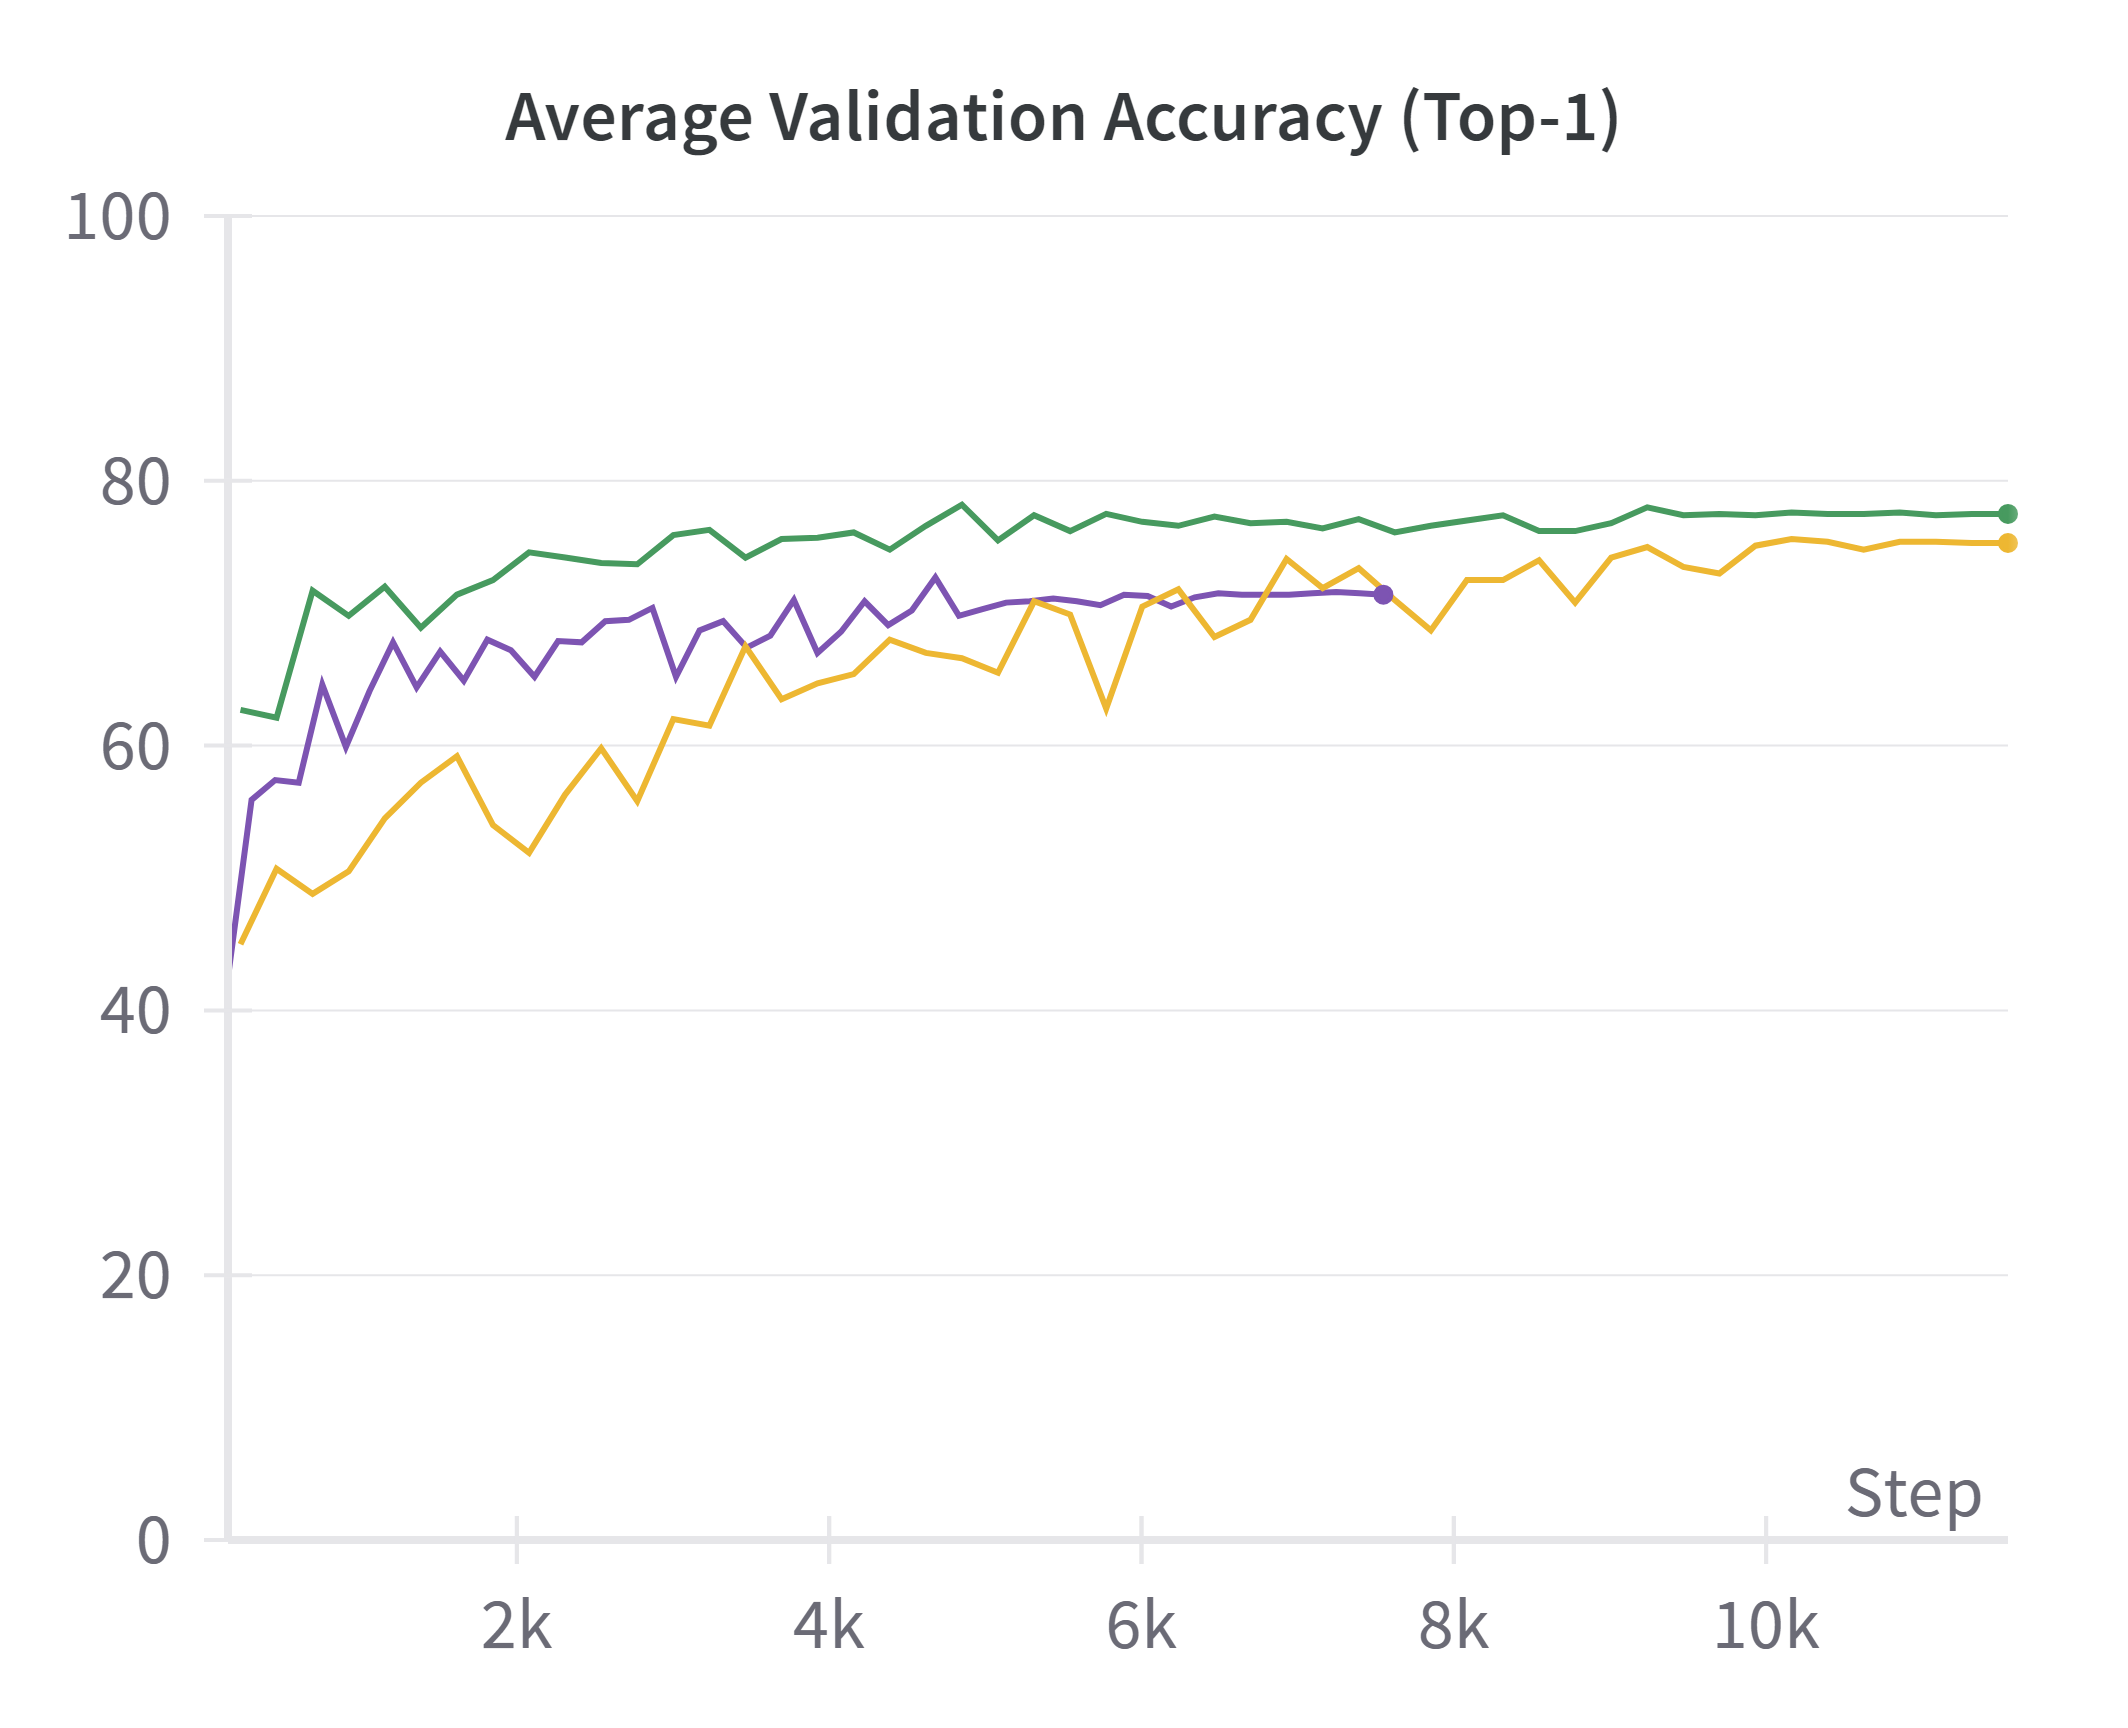
\includegraphics[width=0.5\textwidth]{images/figure_results_supcon-lin_avg-val-acc.png}
	\caption[Trainings- und Validierungs-Accuracy während der linearen Klassifikation.]{Trainings- und Validierungs-Accuracy während der linearen Klassifikation (\textcolor{exp1}{Lila}: Versuch 1, \textcolor{exp2}{Grün}: Versuch 2, \textcolor{exp3}{Gelb}: Versuch 3).}
	\label{fig:supcon-lin-acc}
\end{figure}

% Viel geringere Trainingsgenauigkeit bei Versuch 3, dann ber doch hohe Validierungsgenauigkeit (?)
Ähnliches kann in Bezug auf die Top-1 Accuracy beobachtet werden. Die Trainings-Accuracy ist bei Versuch 3 deutlich niedriger als bei den anderen Versuchen, während die Validierungs-Accuracy ein ähnlich hohes Niveau erreicht. Interessanterweise zeigt sich, dass die schnelle Konvergenz des Trainingsfehlers bzw. der Trainings-Accuracy in Versuchen 1 und 2 das Lernen in gewisser Weise ausbremst, wodurch auf den Validierungsdaten wenig Verbesserung erzielt wird. In Versuch 3 hingegen scheint das Modell auf den Trainingsdaten nicht so schnell zu konvergieren, wodurch die Validierungs-Accuracy stetiger steigt.

\begin{figure}[h]
	\centering
	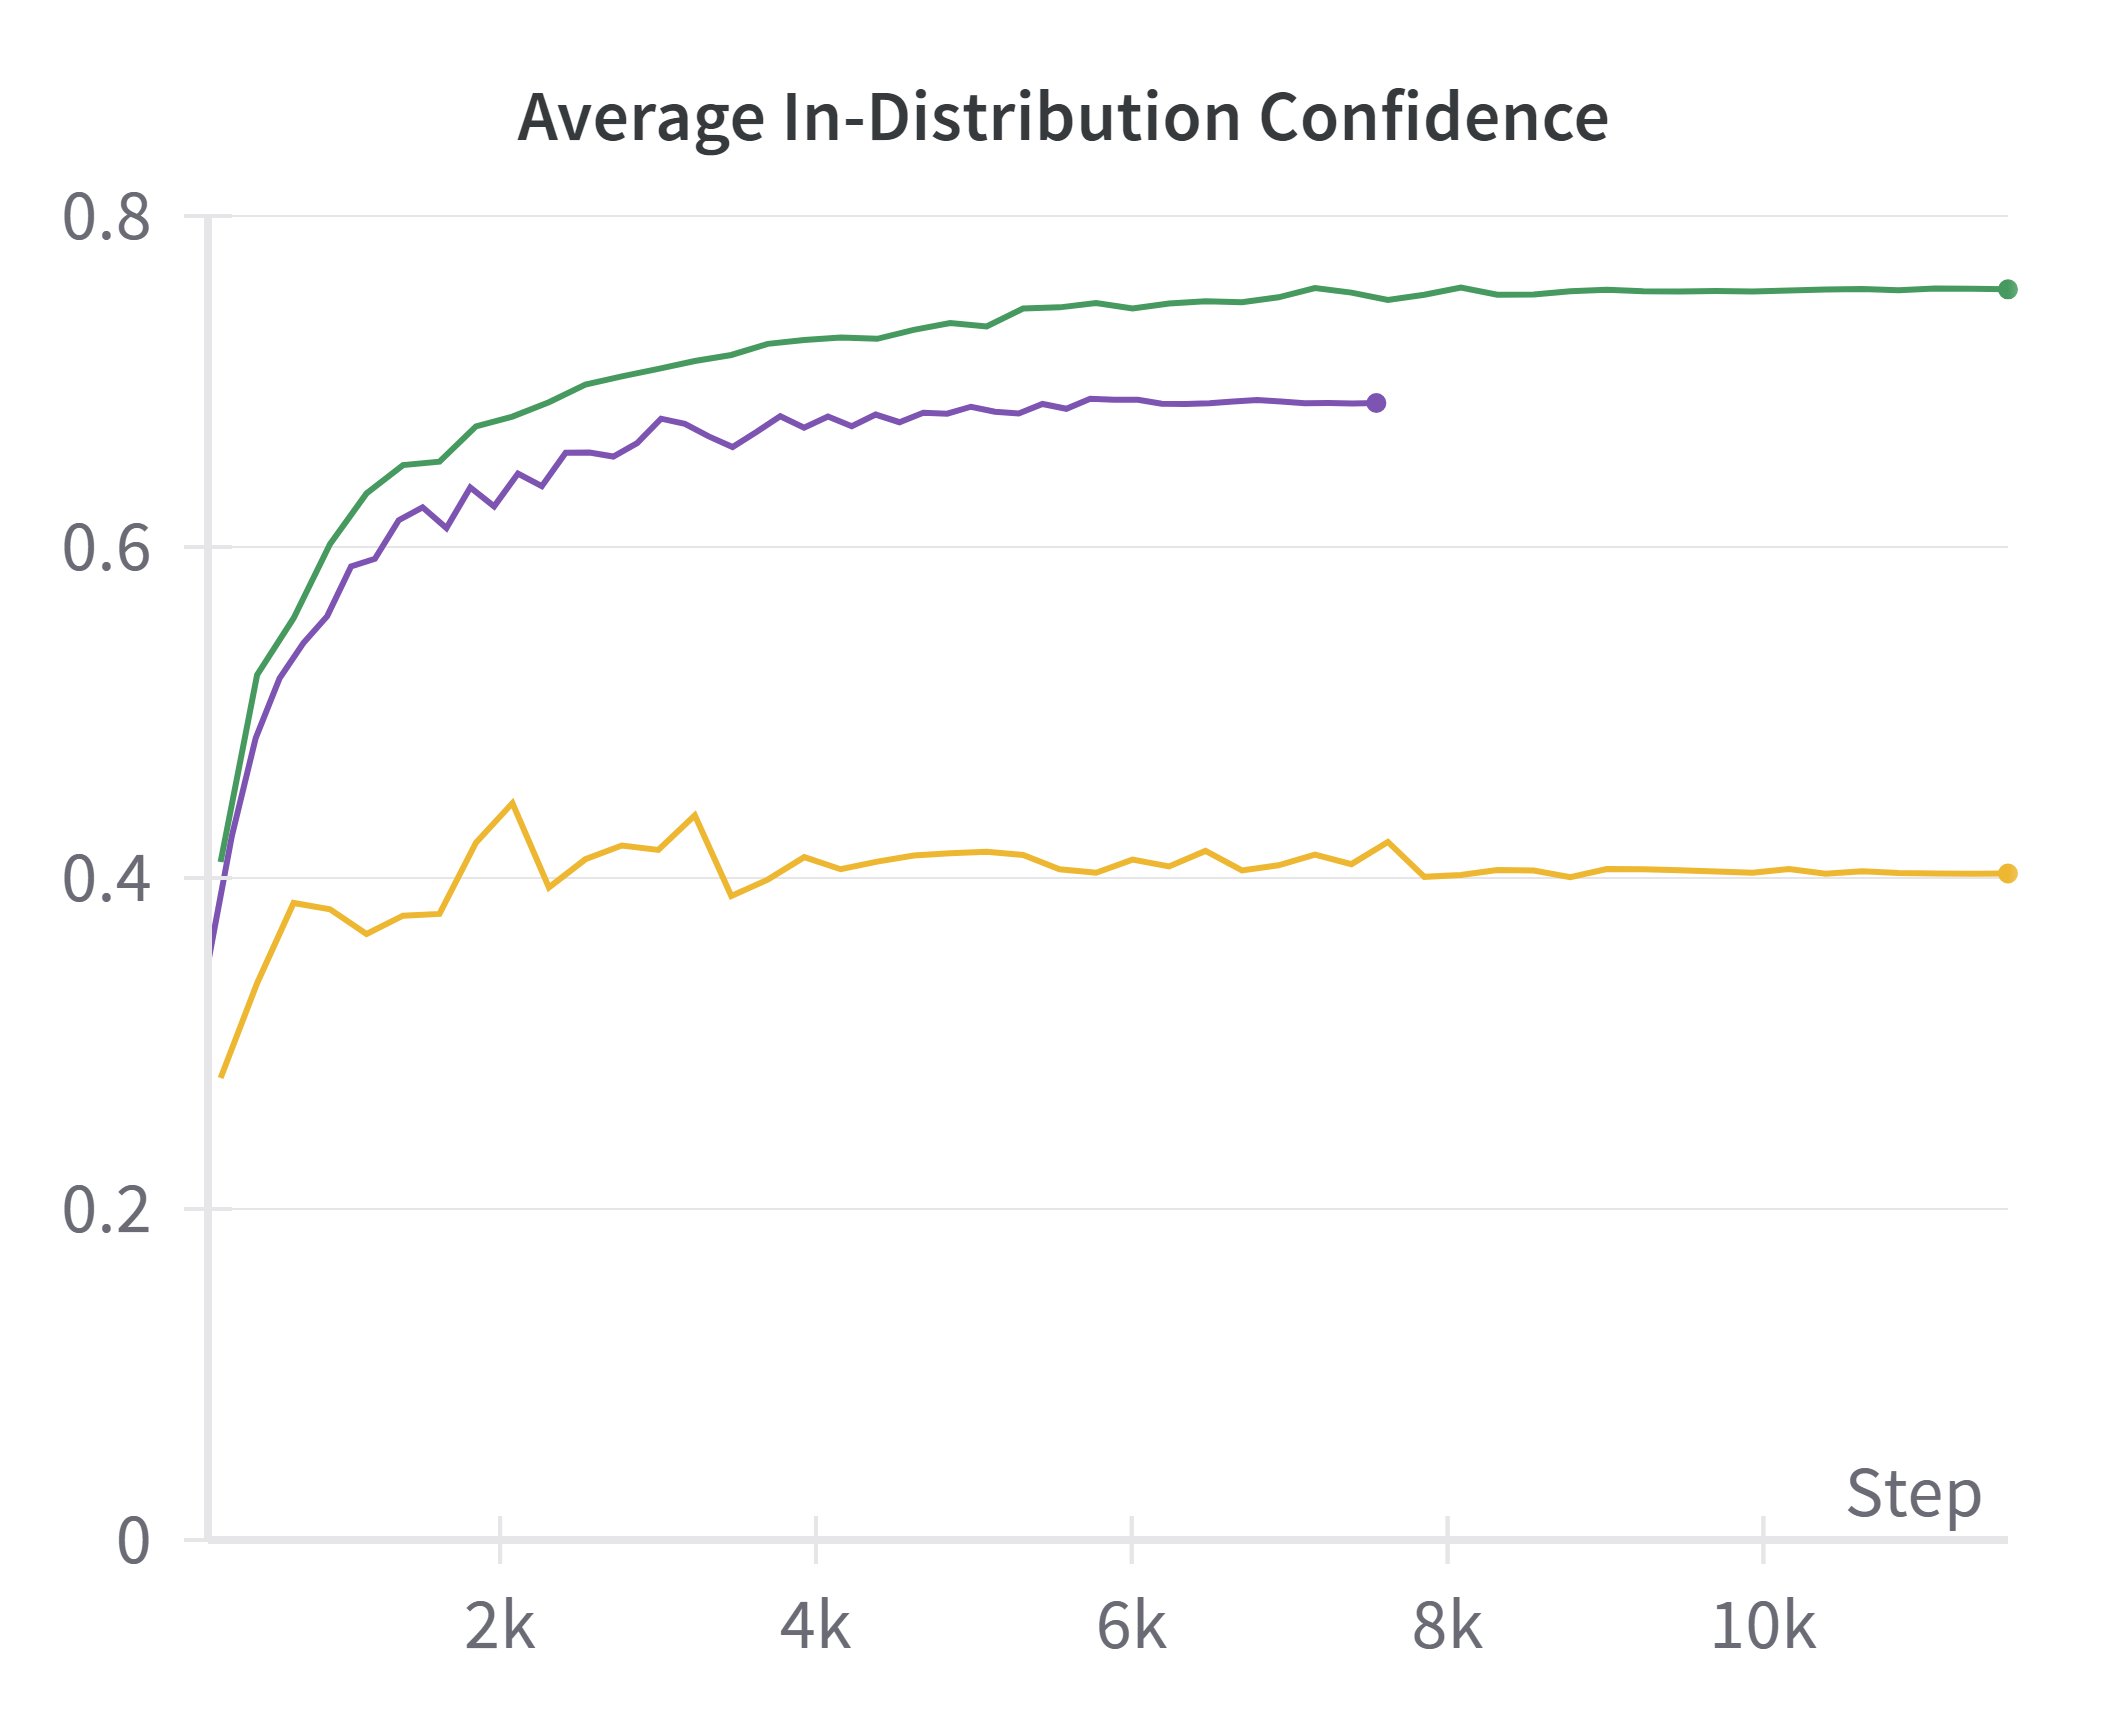
\includegraphics[width=0.5\textwidth]{images/figure_results_supcon-lin_avg-id-conf.png}%
	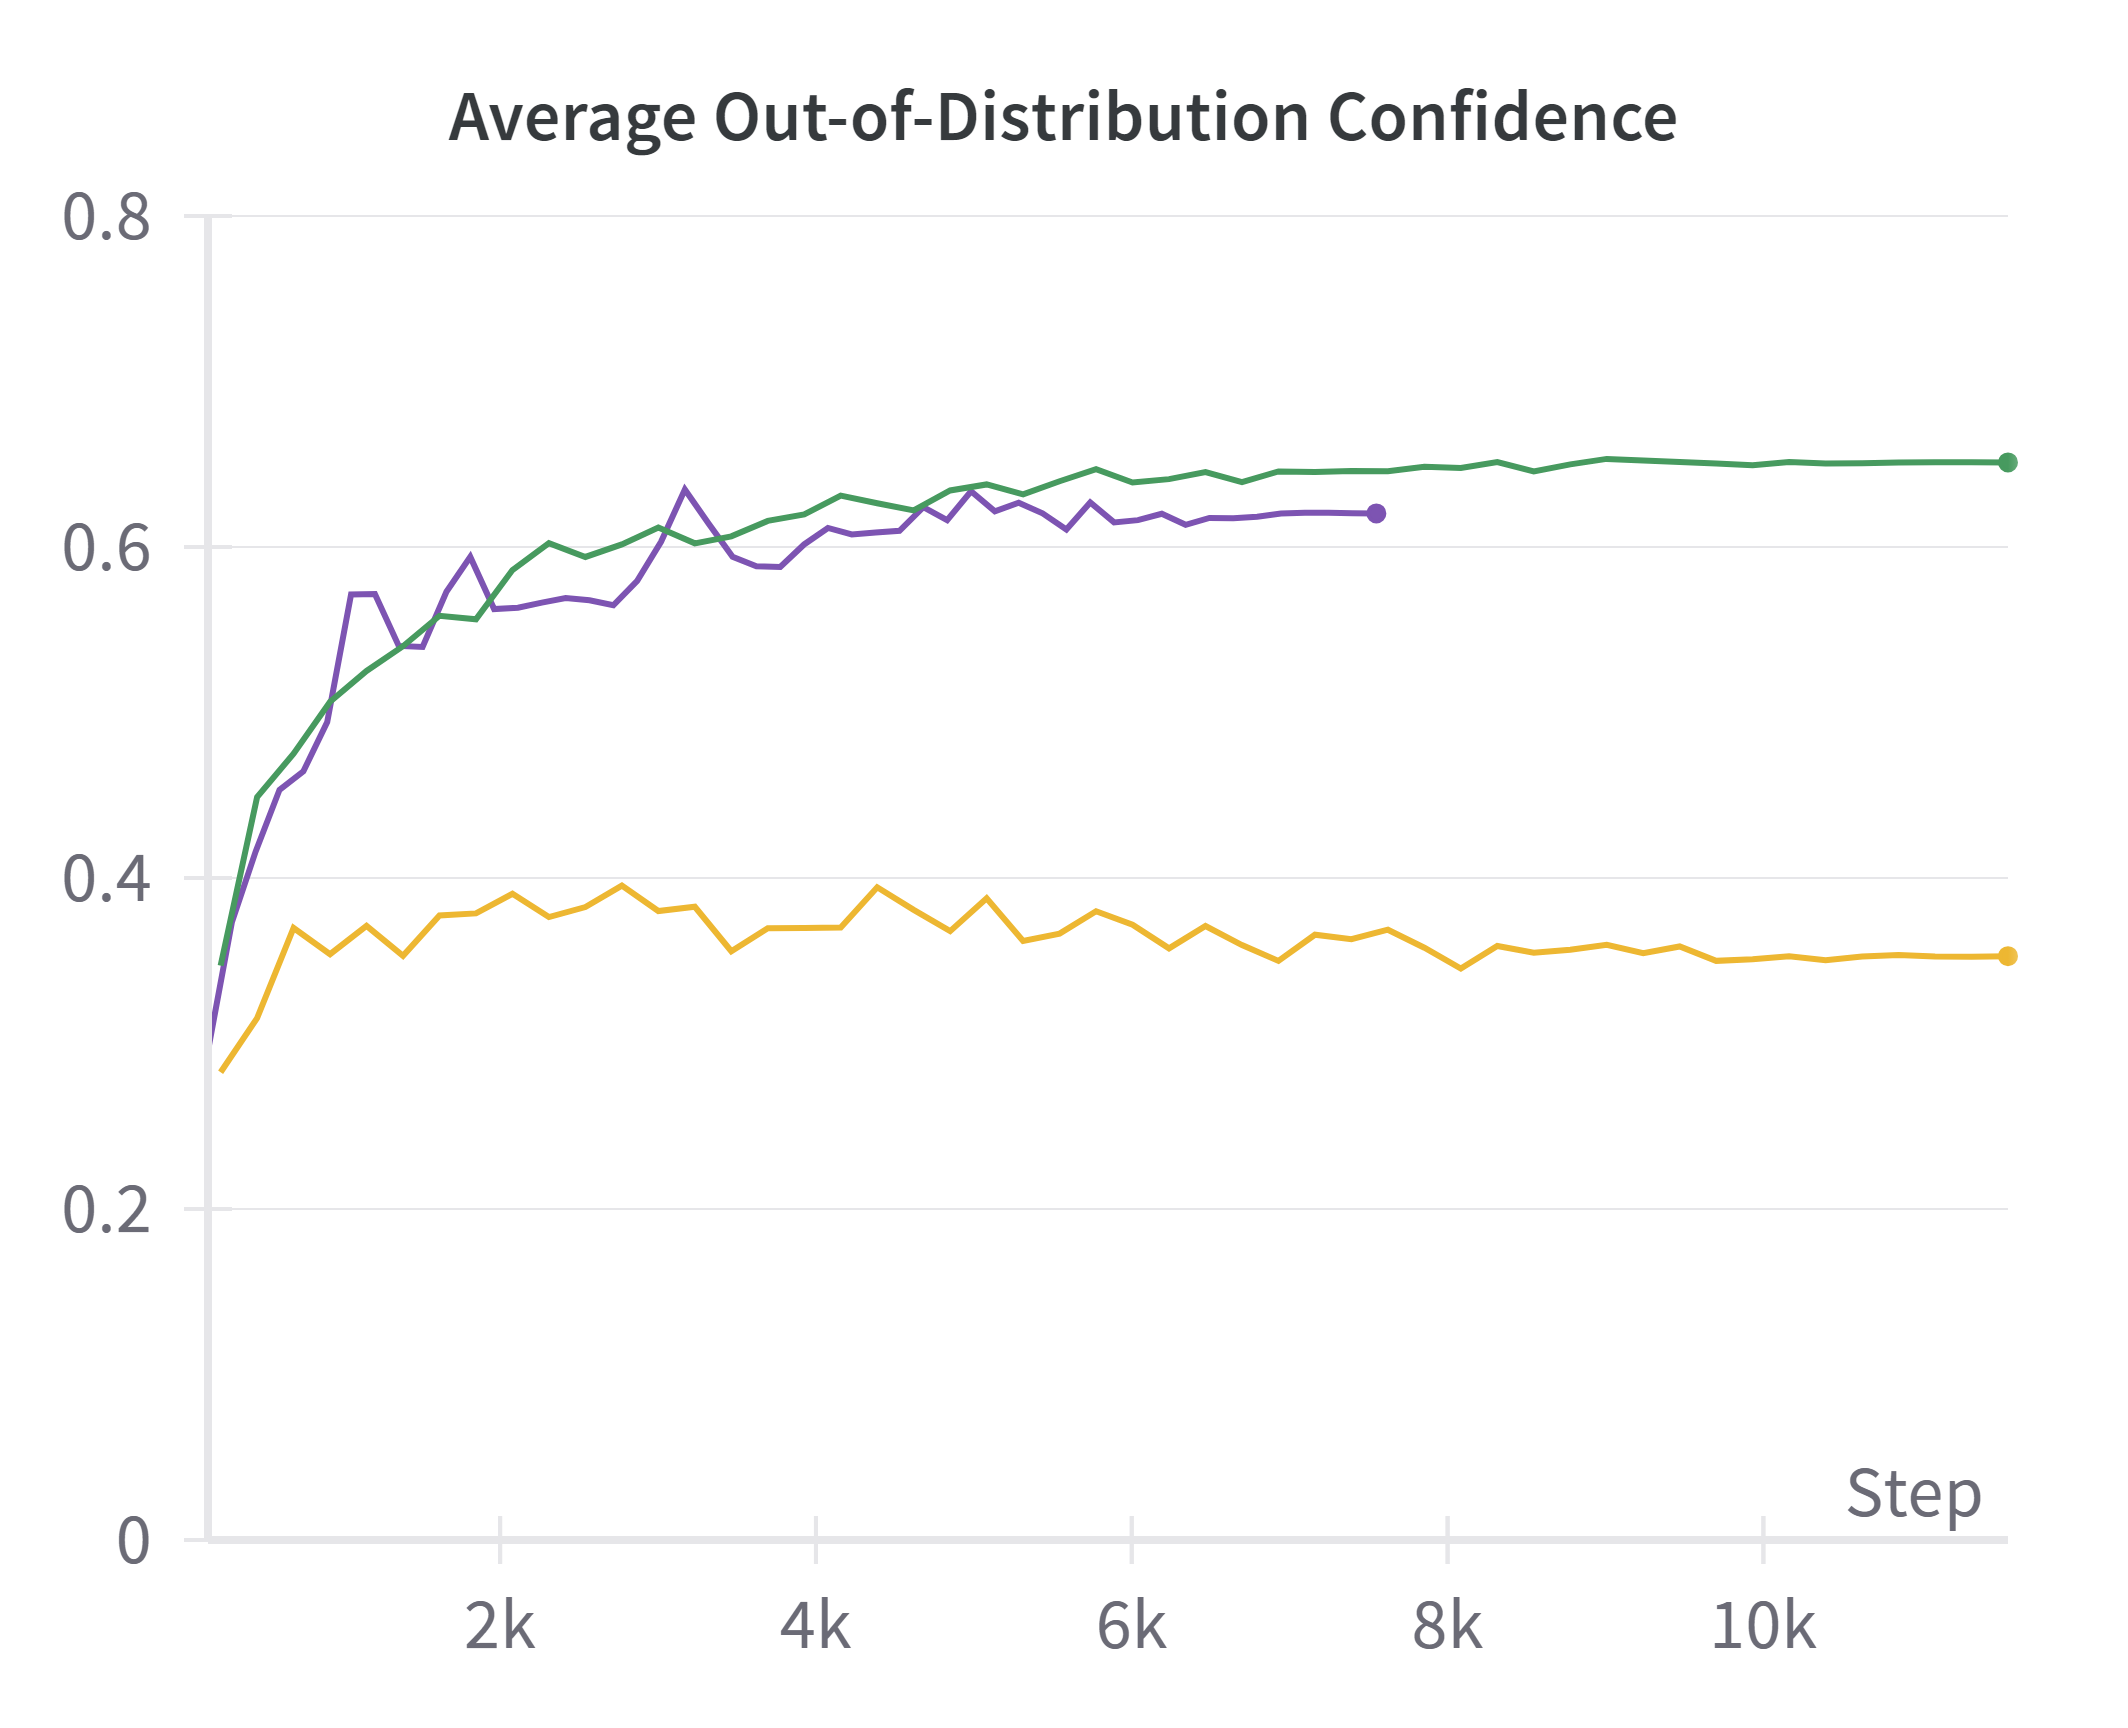
\includegraphics[width=0.5\textwidth]{images/figure_results_supcon-lin_avg-ood-conf.png}
	\caption[ID- und OOD-Confidence während der linearen Klassifikation.]{ID- und OOD-Confidence während der linearen Klassifikation (\textcolor{exp1}{Lila}: Versuch 1, \textcolor{exp2}{Grün}: Versuch 2, \textcolor{exp3}{Gelb}: Versuch 3).}
	\label{fig:supcon-lin-ood-detection}
\end{figure}

% Versuch 3 mit Abstand die niedrigsten Confidence-Werte (ID & OOD), und sogar den niedrigsten Abstand
Die ID-Confidence ist bei Versuch 2 deutlich höher als bei Versuch 1, während die OOD-Confidence bei beiden Versuchen vergleichbar bleibt. Versuch 3 zeigt jedoch die niedrigsten Confidence-Werte, sowohl für ID als auch für OOD, und hat auch den niedrigsten Abstand zwischen den beiden Werten. In der Trainingskurve ist dabei kaum Konvergenz zu erkennen.

\section{Vergleich der Ergebnisse} \label{sec:results-comparison}

% Einleitung
Als Grundlage für die Diskussion und Beantwortung der Forschungsfragen werden die finalen Ergebnisse nach Durchlaufs des Trainings noch einmal gegenübergestellt. Es werden konkret die Messungen mit und ohne In-Distribution-Augmentationen (im Bezug auf die erste Forschungsfrage) bzw. mit und ohne Near Out-of-Distribution-Augmentationen (im Bezug auf die zweite Forschungsfrage) verglichen. Dabei wird auf die Klassifikations-Performance (Accuracy) und die Out-of-Distribution-Detektion (ID-/OOD-Confidence) eingegangen.

\subsection{Mit und ohne In-Distribution-Augmentationen} \label{subsec:results-comparison-id}

In Bezug auf die erste Forschungsfrage werden Versuche 1 und 2 verglichen. In Versuch 1 wurden sowohl Contrastive Pre-Training als auch lineare Klassifikation ohne jegliche Augmentationen durchgeführt, während in Versuch 2 in beiden Schritten In-Distribution-Augmentationen verwendet wurden.

% Metriken
Die Einführung der In-Distribution-Augmentationen hatte insgesamt einen positiven Effekt auf die Klassifikations-Performance der Modelle. Die Top-1 Accuracy konnte von 71.4\% auf 77.5\% gesteigert werden, was eine signifikante Verbesserung darstellt. Die ID-Confidence stieg von 0.69 auf 0.76, während die OOD-Confidence von 0.62 auf 0.65 anstieg. Der Abstand zwischen ID- und OOD-Confidence erhöhte sich von 0.07 auf 0.11, was effektiv eine Verbesserung der OOD-Detektion darstellt.

\subsection{Mit und ohne Near Out-of-Distribution-Augmentationen} \label{subsec:results-comparison-ood}

In Bezug auf die zweite Forschungsfrage werden Versuche 2 und 3 verglichen. In Versuch 2 wurde sowohl das Contrastive Pre-Training als auch die lineare Klassifikation mit In-Distribution-Augmentationen durchgeführt. In Versuch 3 wurden im Pre-Training der Repräsentationen zusätzlich Near Out-of-Distribution-Augmentationen verwendet.

% Metriken
Die Klassifikations-Performance der Modelle verschlechterte sich durch die Near Out-of-Distribution-Augmentationen. Die Top-1 Accuracy sank von 77.5\% auf 75.3\% und die ID-Confidence fiel drastisch von 0.76 auf 0.40. Die OOD-Confidence fiel ebenfalls von 0.65 auf 0.35, dabei wurde der Abstand zwischen ID- und OOD-Confidence aber von 0.11 auf 0.05 verringert, was eine Verschlechterung der OOD-Detektion bedeutet.